%!TEX root = informe.tex
\addcontentsline{toc}{chapter}{Plano modelo adoquín Holanda 6}

\begin{figure}[!htb]
\centering
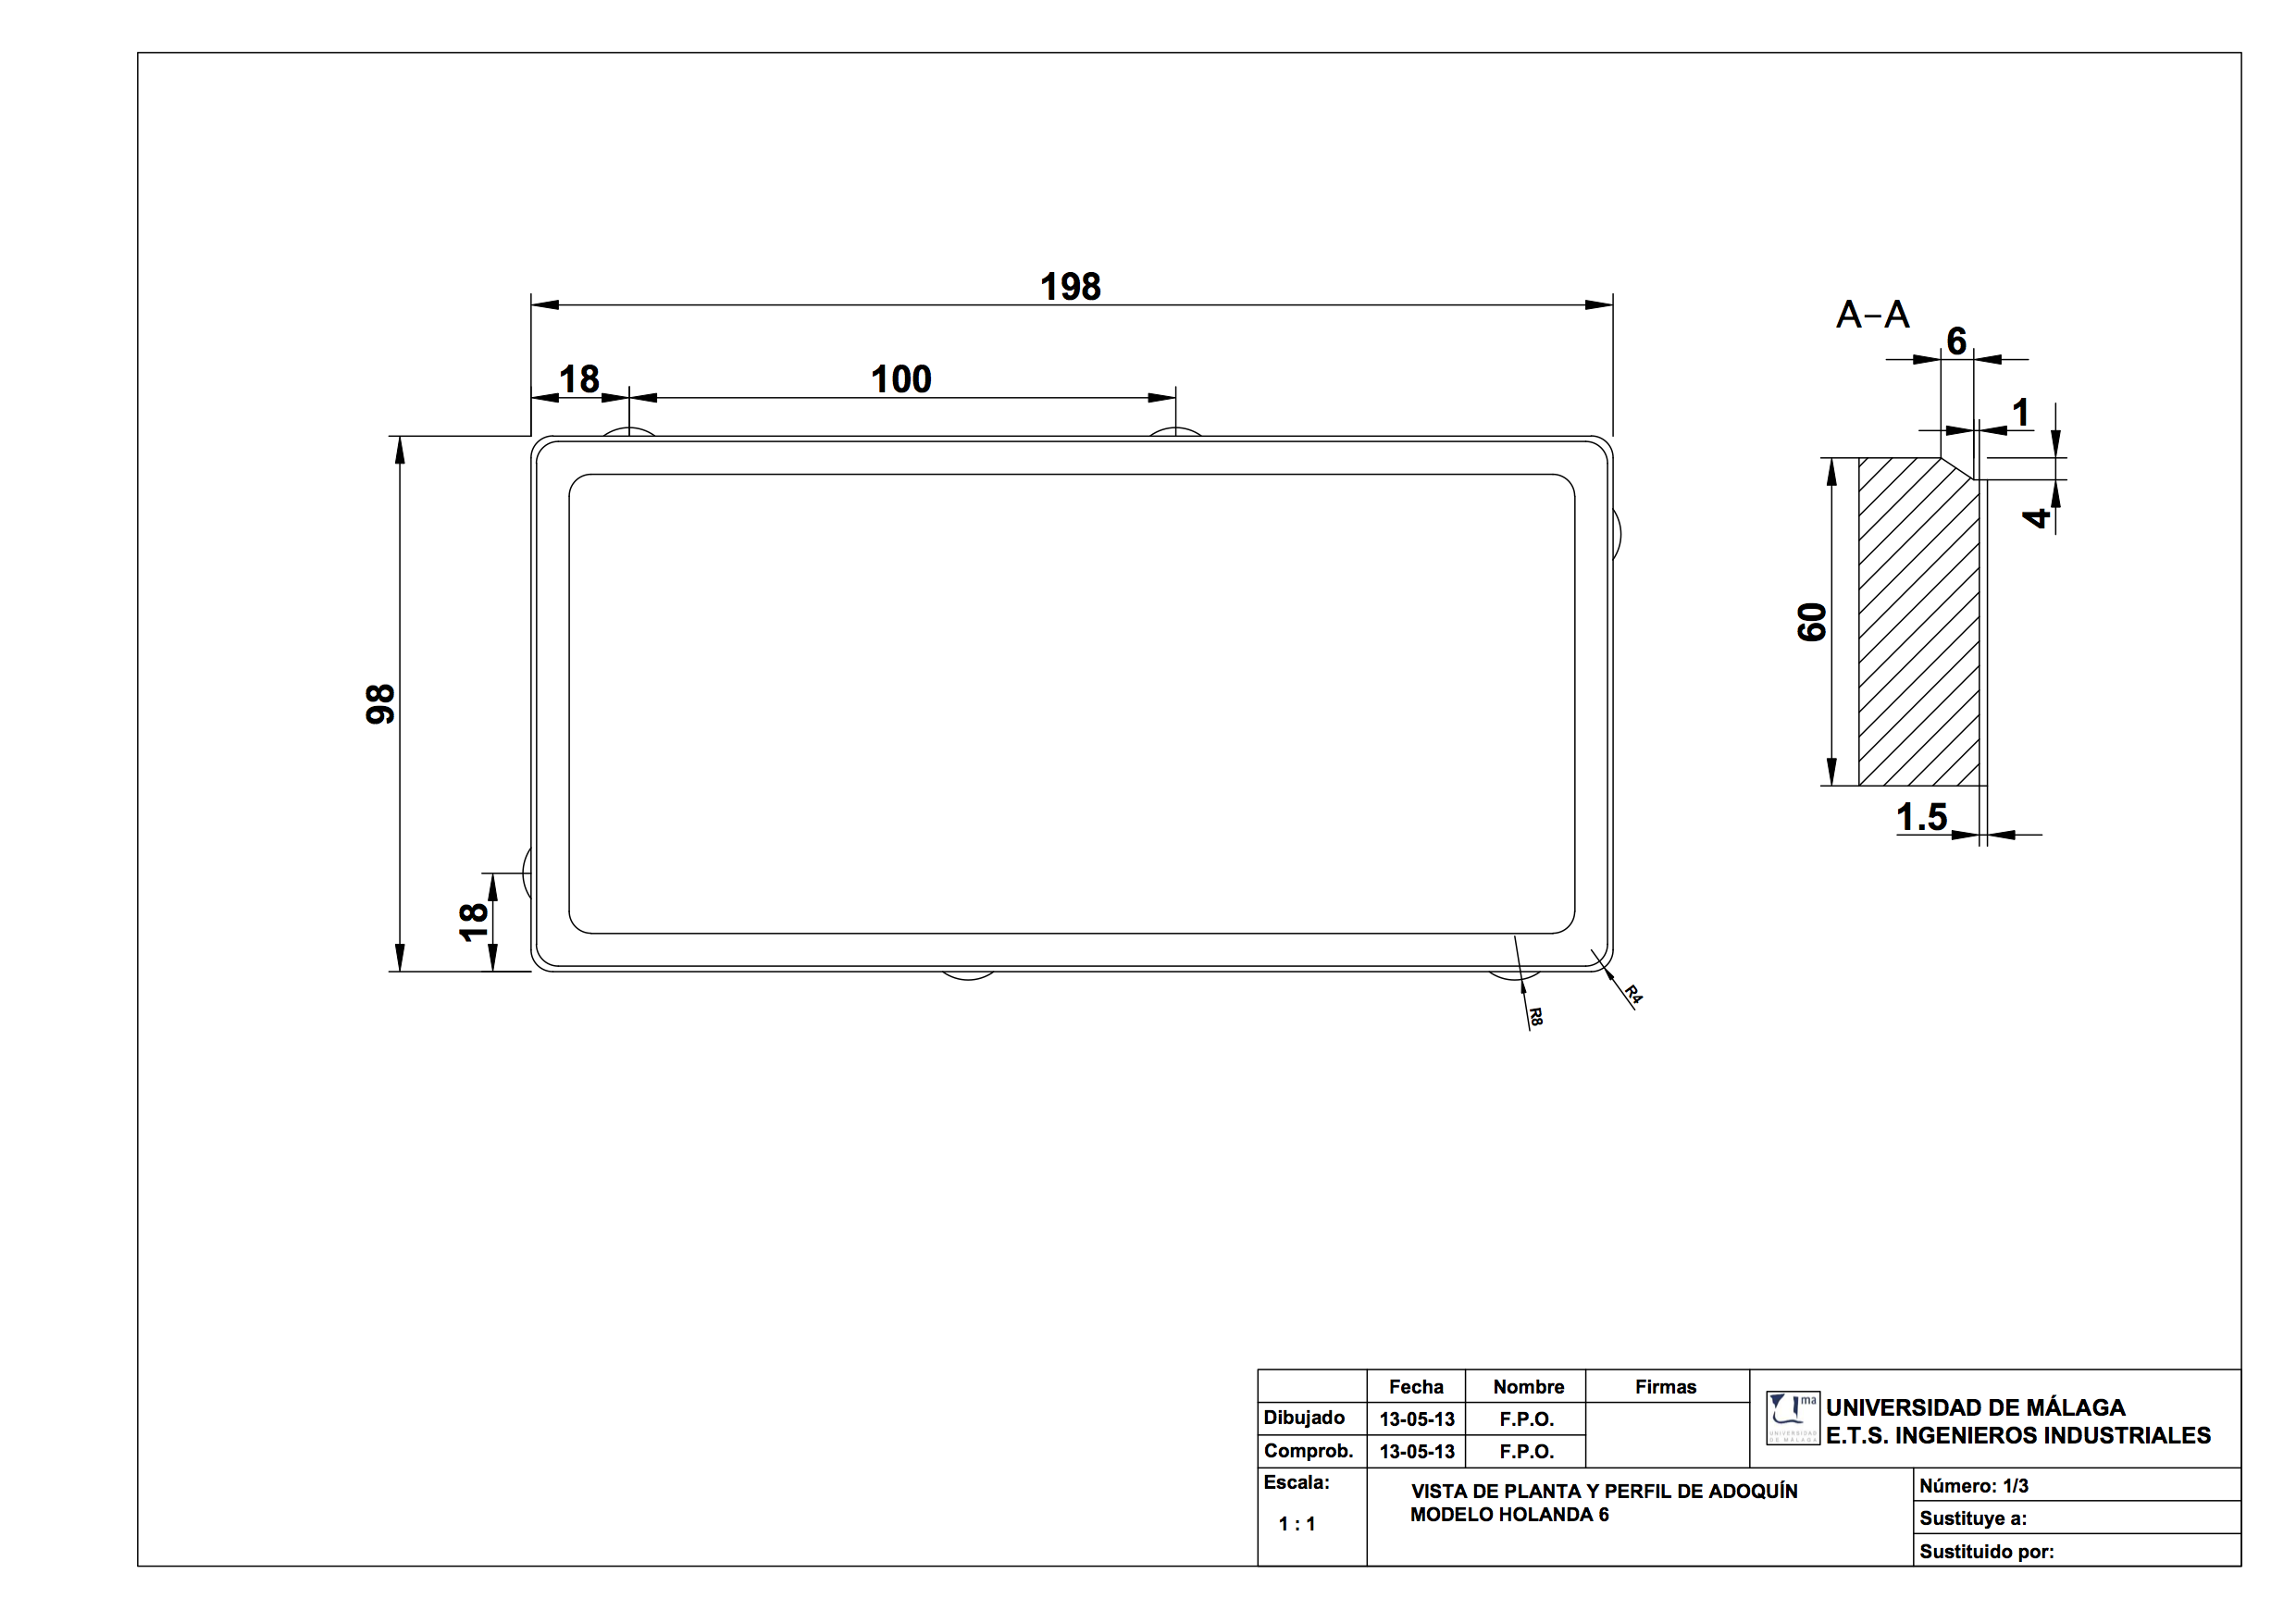
\includegraphics[angle=90,width=13.5cm]{plano_adoquin.png}
% \caption{Plano modelo adoquín Holanda 6.}
% \label{fig:planoadoquin}
\end{figure}

\newpage
\addcontentsline{toc}{chapter}{Plano molde adoquín Holanda 6}

\begin{figure}[!htb]
\centering
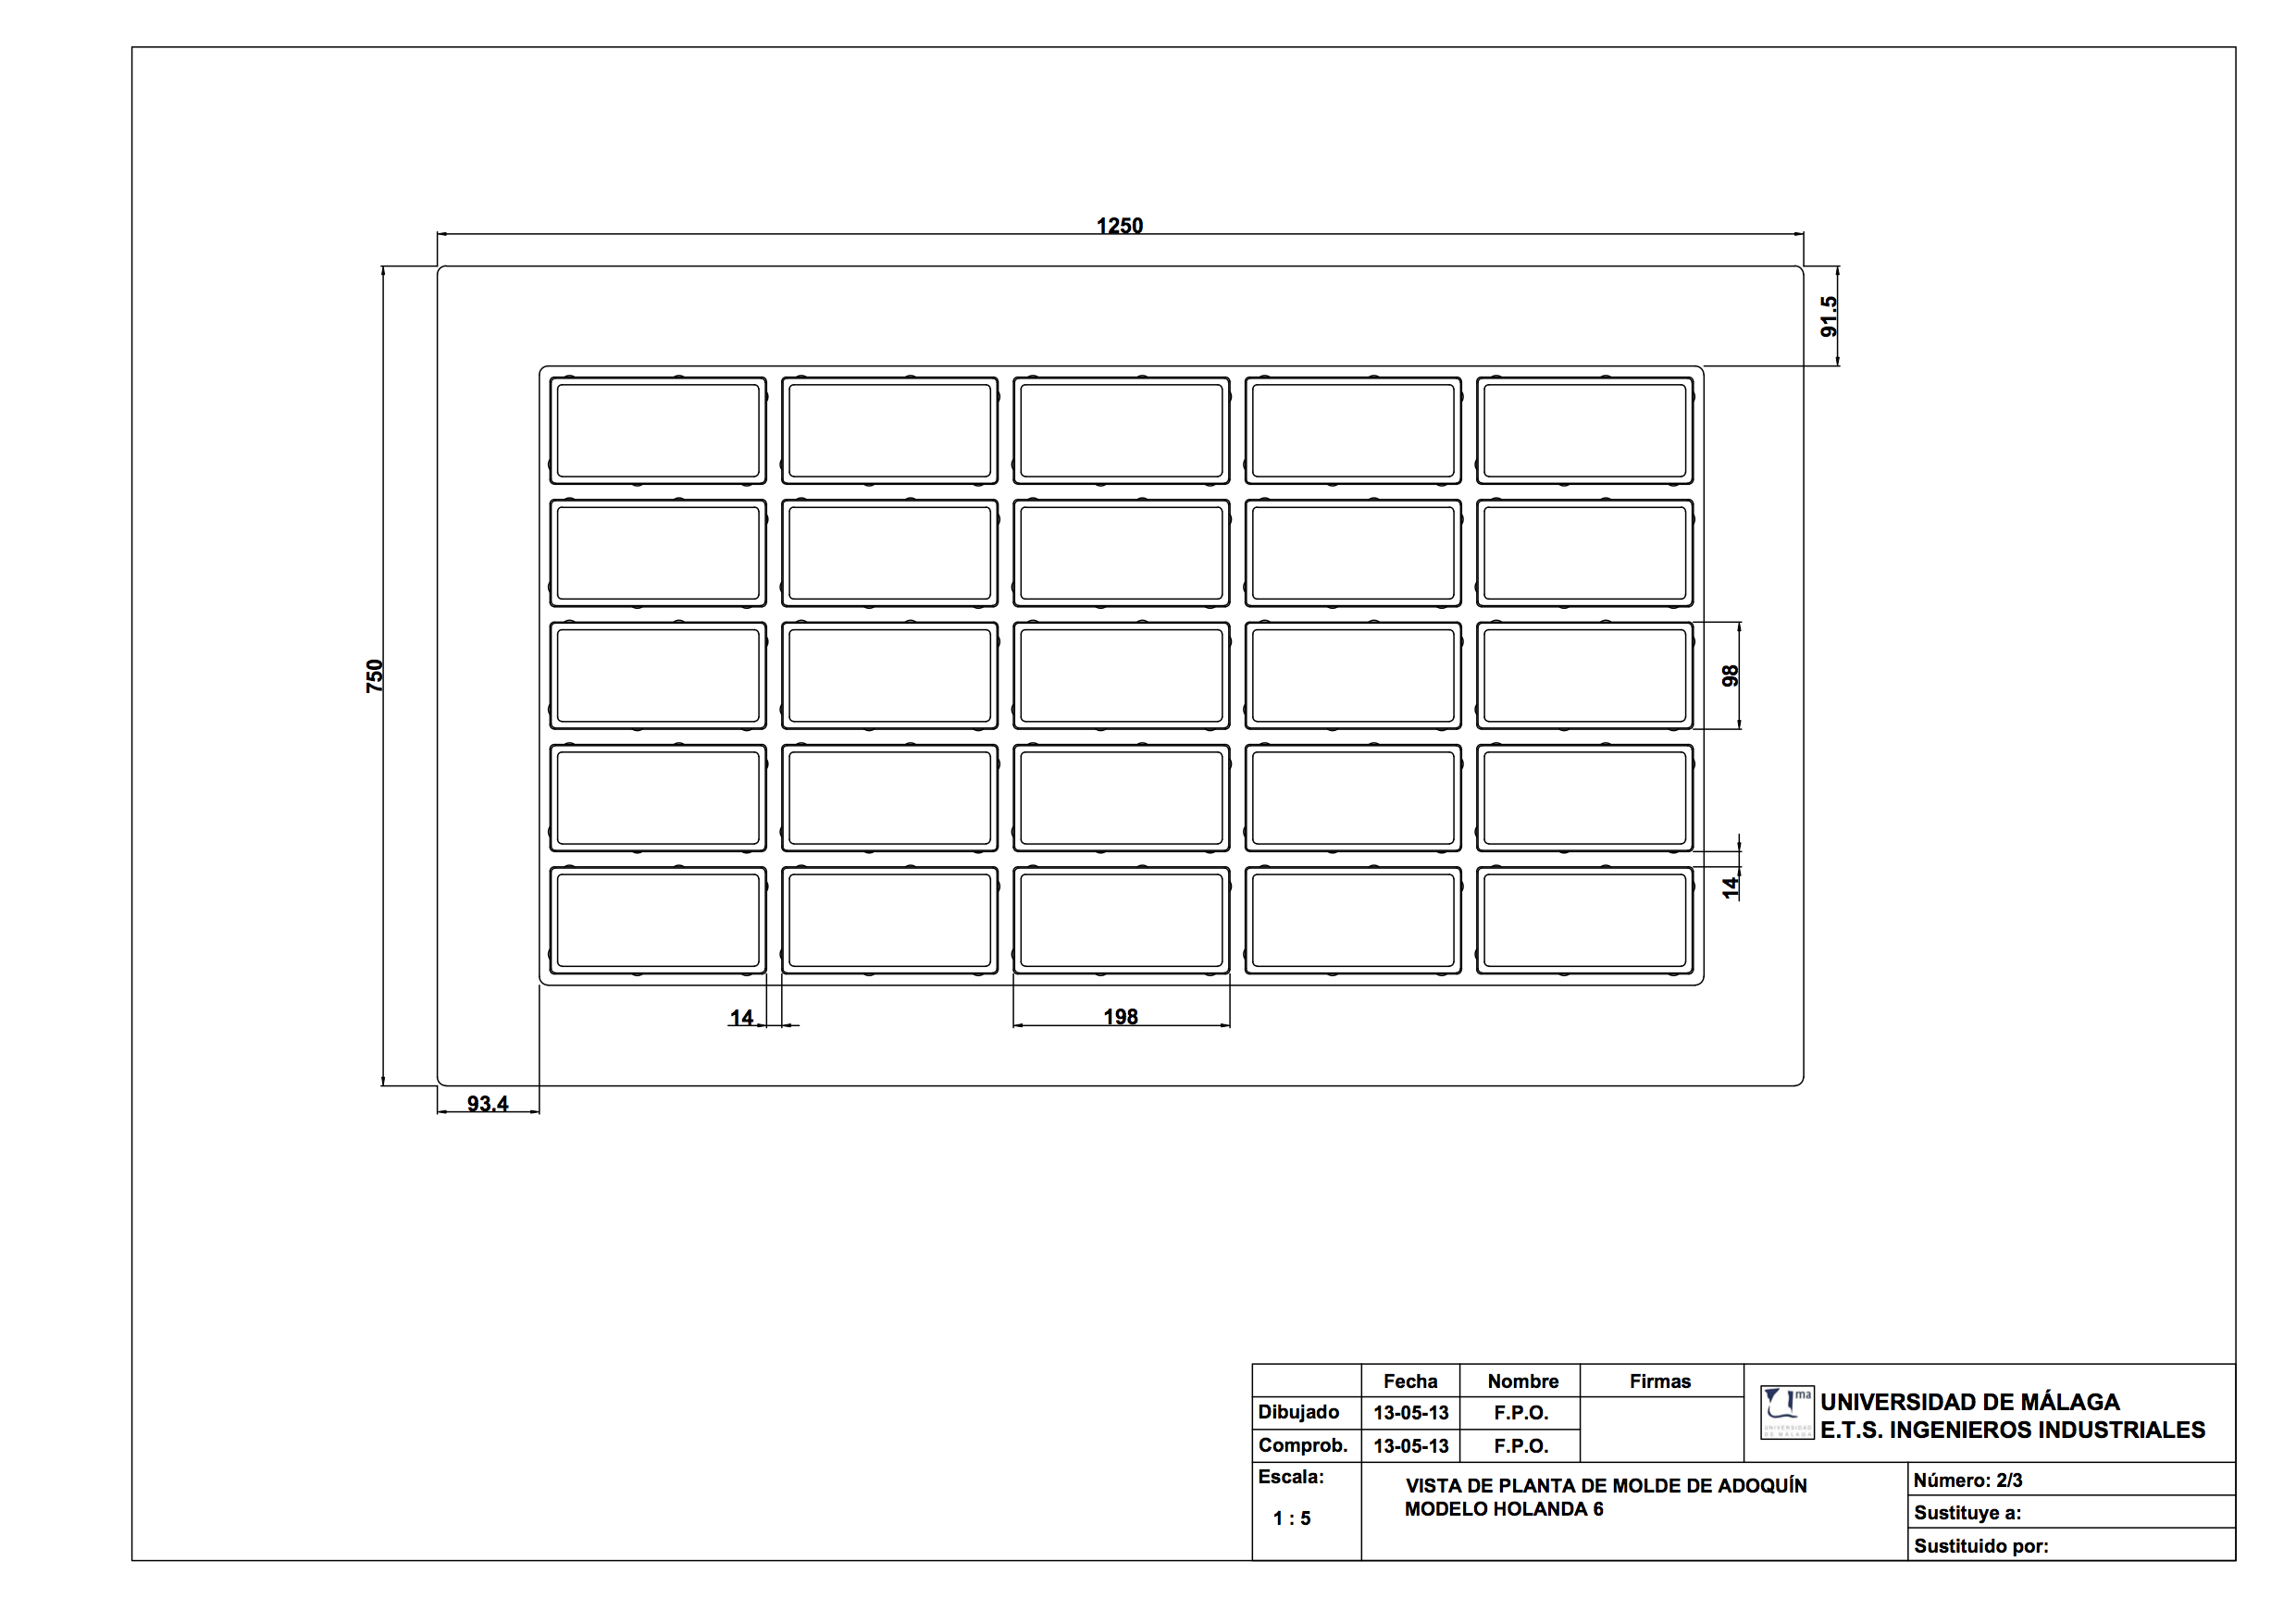
\includegraphics[angle=90,width=13.5cm]{plano_molde.png}
% \caption{Plano molde adoquín Holanda 6.}
% \label{fig:planomolde}
\end{figure}

\newpage
\addcontentsline{toc}{chapter}{Plano de instalaciones}

\begin{figure}[!htb]
\centering
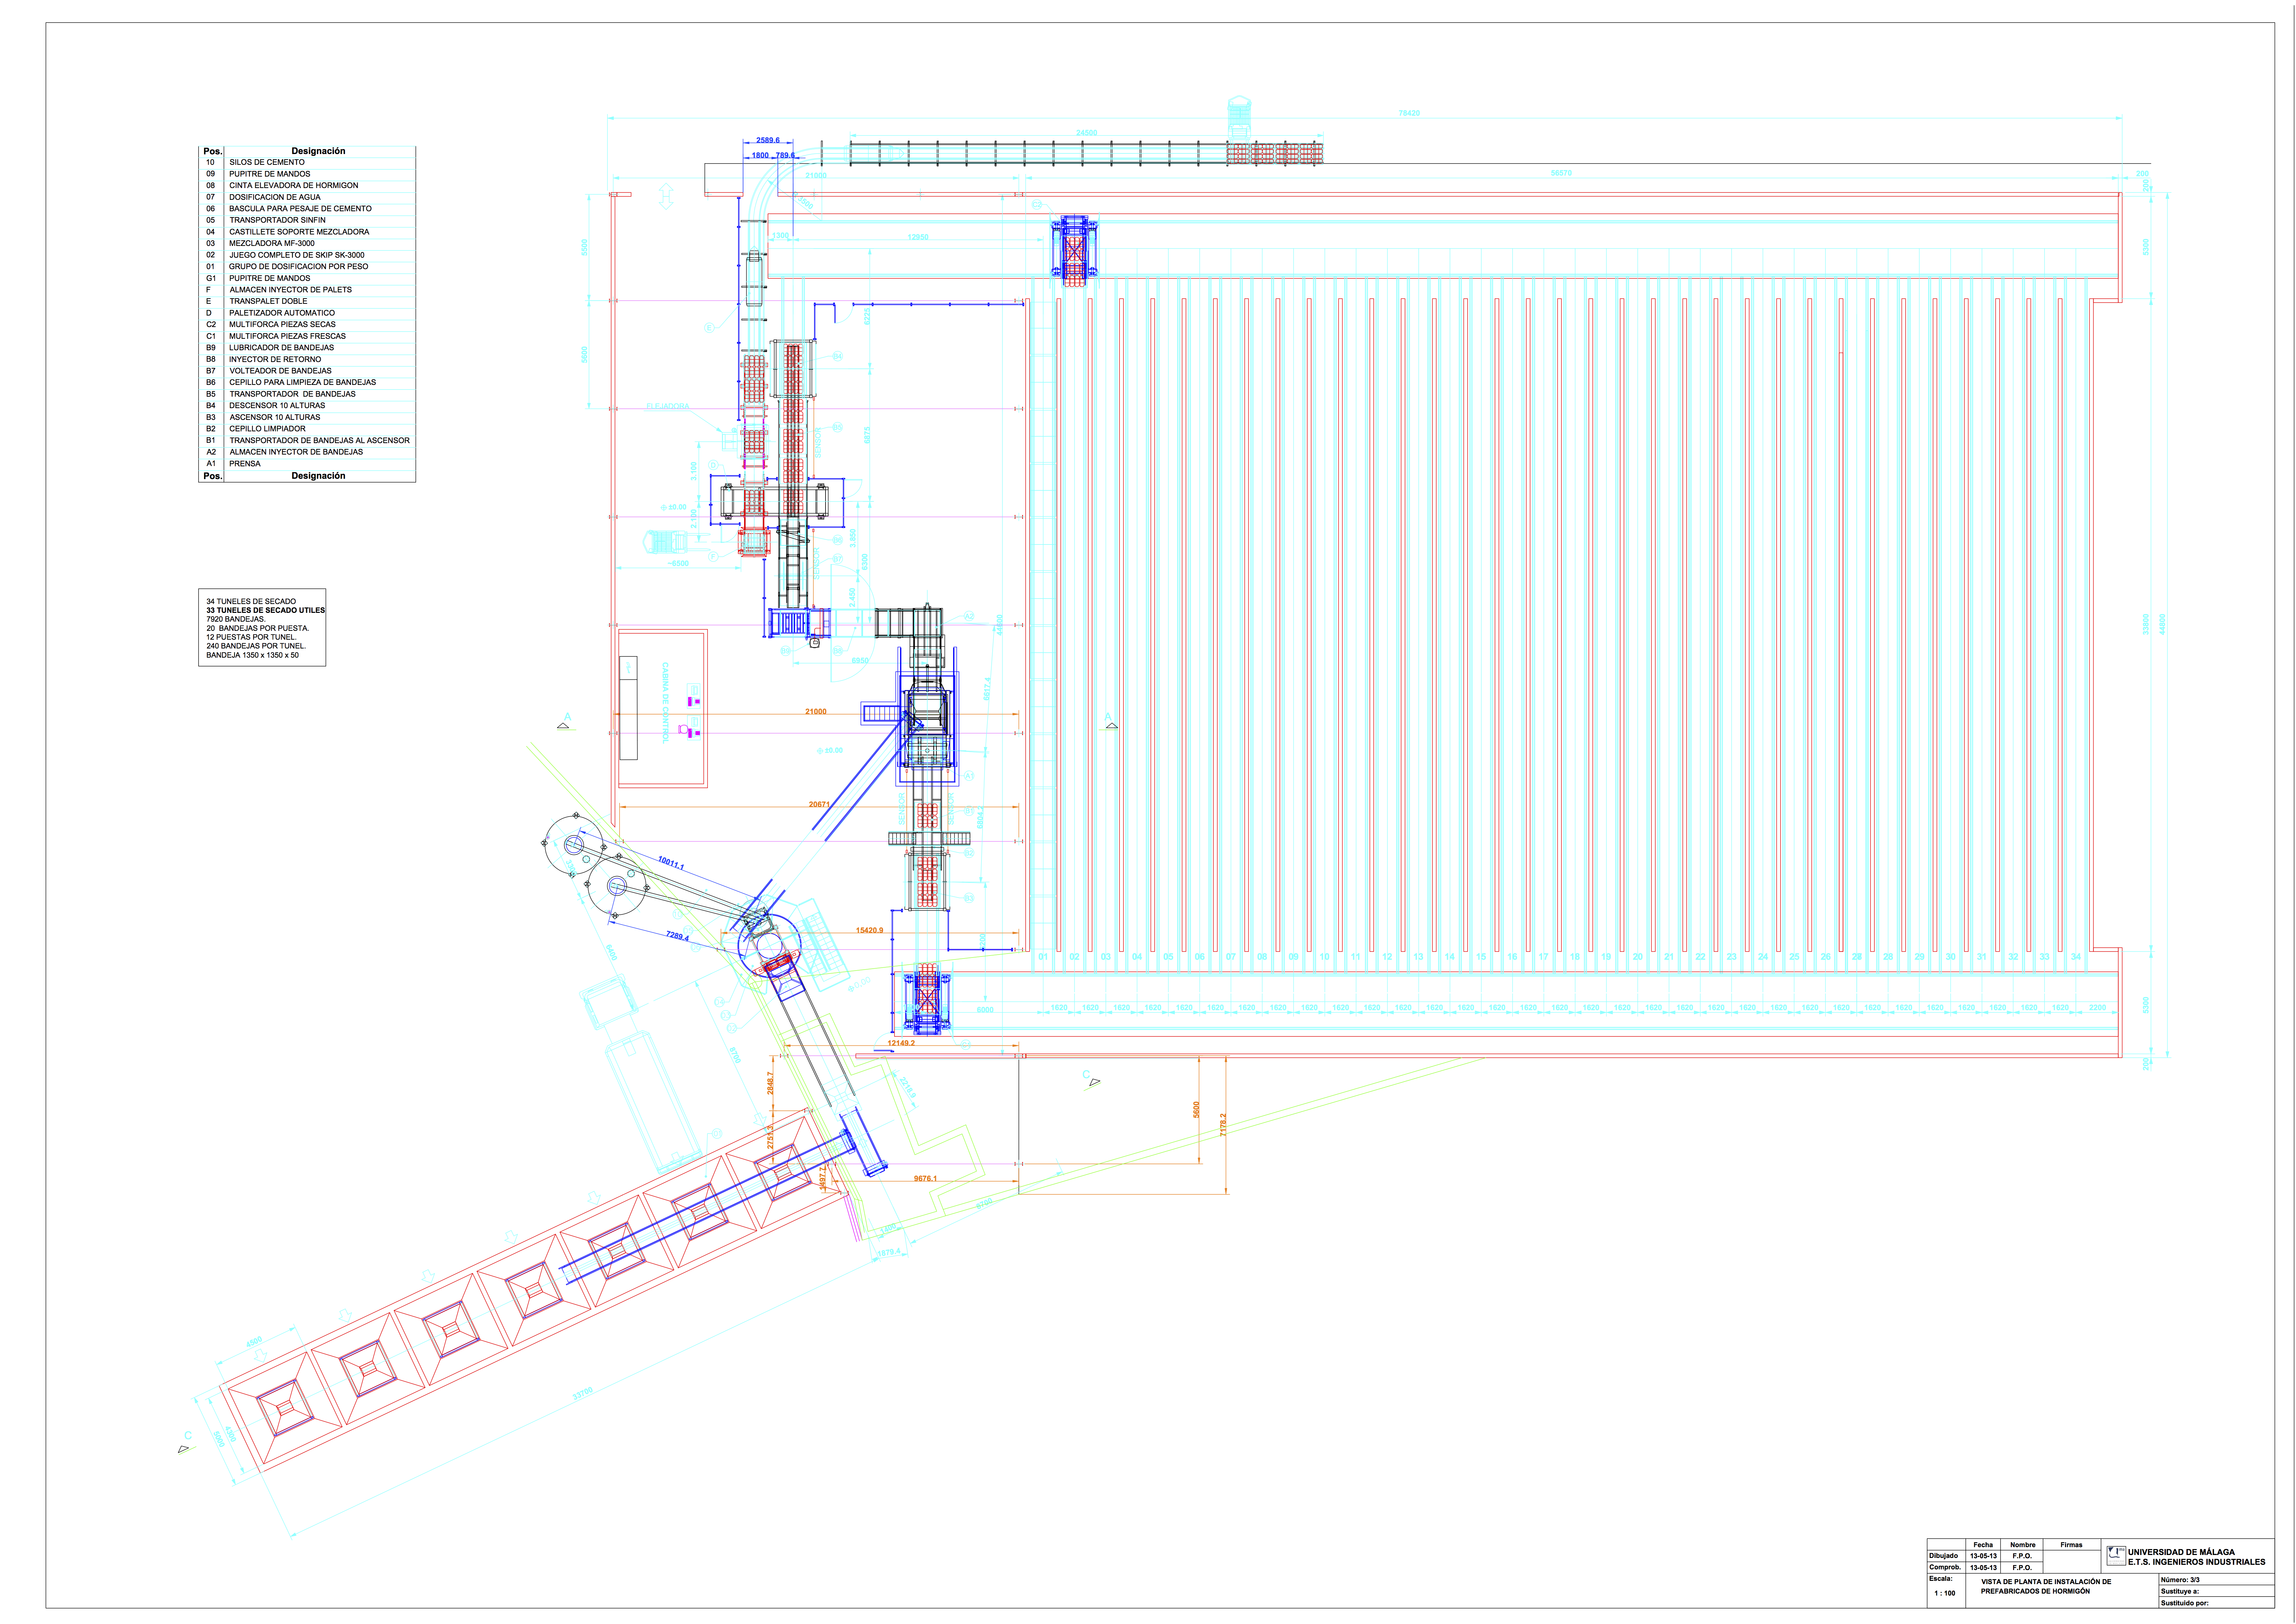
\includegraphics[angle=90,width=13.5cm]{plano_nave.png}
% \caption{Plano de instalaciones.}
% \label{fig:planonave}
\end{figure}
